% Just The Docs Front Matter
% title: Pine Island Glacier Stochastic Forcing (StISSM)
% parent: Tutorials
% has_children: false
% has_toc: false

\subsection{Pine Island Glacier Stochastic Forcing (StISSM)} \label{sec:using-issm-tutorials-pigstissm}
\subsubsection{Goals} %{{{
\begin{itemize}
	\item Introduction to the use of the stochastic capabilities implemented in ISSM (StISSM)
	\item Model Pine Island Glacier as in previous tutorials, but with stochastic forcings
\end{itemize}
%}}}

\subsubsection{Introduction}%{{{
The main goals of this tutorial are 1) to become familiar with the use of StISSM, 2) to learn how to parameterize stochastic variables of the model, and 3) to launch transient stochastic simulations. The first steps follow what was done in previous tutorials: setting up the model domain and general configuration for the Pine Island Glacier. The organization of the tutorial is as follows:
\begin{itemize}
	\item Step 1: Generate a model mesh
	\item Step 2: Set up the ice and ocean masks
	\item Step 3: Parameterization of the model
	\item Step 4: Set up the stochastic SMB parameterization
	\item Step 5: Transient run
	\item Step 6: Set up the stochastic calving parameterization
	\item Step 7: Second transient run starting from the results of the first one
\end{itemize}
Files needed for this tutorial can be found in \lstinlinebg|trunk/examples/StISSM/|. The \lstinlinebg|runme.m| file contains the structure of the overall simulation, while the .par file includes most parameters needed for the model setup. The \lstinlinebg|.exp| files are domain files that define geometric boundaries of the simulation. Observed datasets needed for the parameterization also need to be 
%__@LATEX_ONLY_START@__
\hyperref[sec:using-issm-tutorials-datasets]{downloaded}.
%__@LATEX_ONLY_END@__
%__@MARKDOWN_ONLY_START@__
% <a href="datasets">downloaded</a>.
%__@MARKDOWN_ONLY_END@__
%}}}

\subsubsection{Mesh}%{{{
This step follows what is done in the Pine Island Glacier tutorial. We simply set up the model mesh from the exp files. Set \lstinlinebg|step = 1| in the \lstinlinebg|runme.m| file to execute it.
\begin{figure}
	\begin{center}
		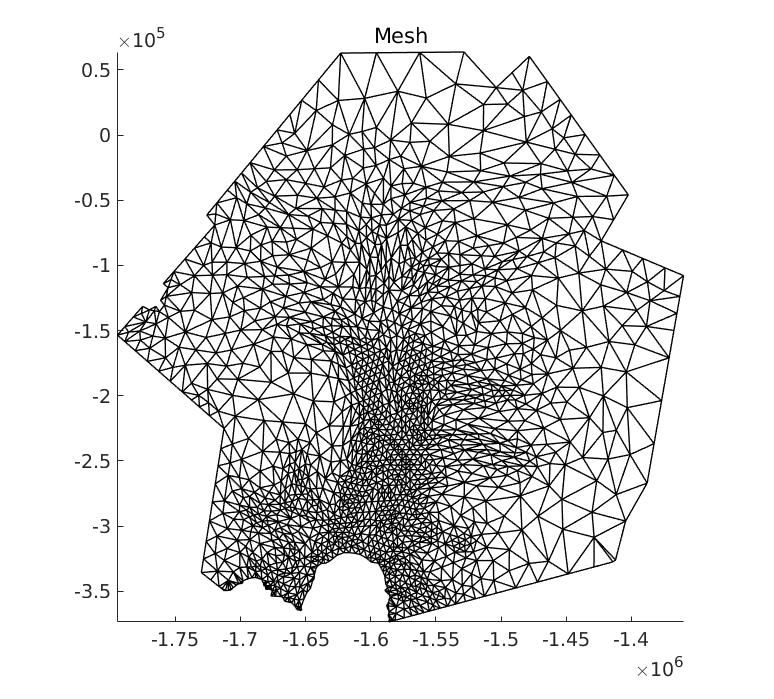
\includegraphics[width=\textwidth]{\assetsParentPath/assets/img/using-issm/tutorials/pigstissm/fig1Mesh.jpg}
	\end{center}
\end{figure}
%}}}

\subsubsection{Mask}%{{{
This step follows what is done in the Pine Island Glacier tutorial. We define the masks where ice is present/absent and where ice is grounded/floating. Set \lstinlinebg|step = 2| in the \lstinlinebg|runme.m| file to execute it.
\begin{figure}
	\begin{center}
		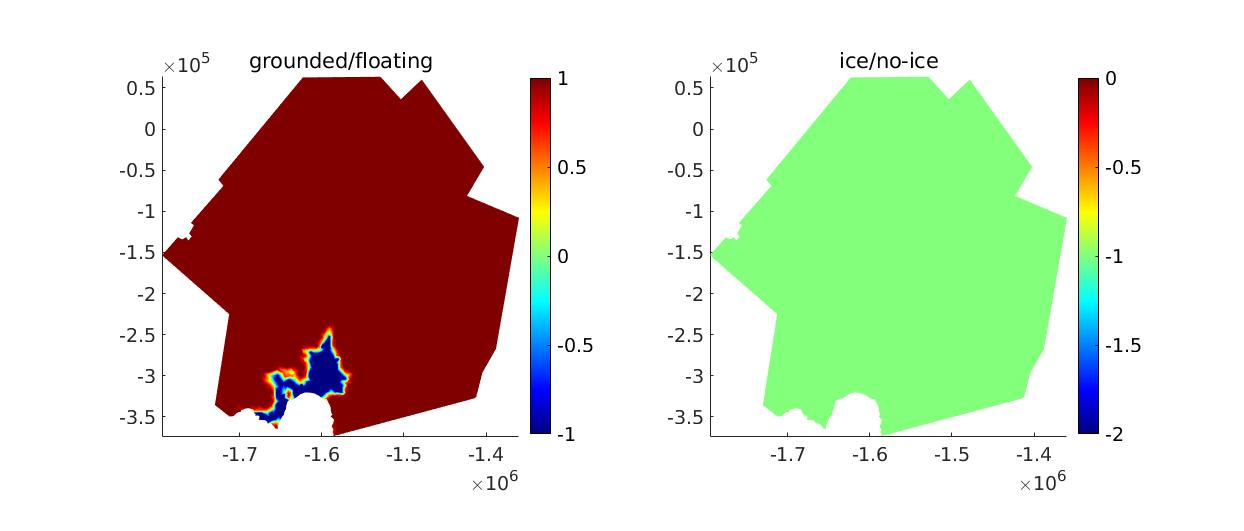
\includegraphics[width=\textwidth]{\assetsParentPath/assets/img/using-issm/tutorials/pigstissm/fig2Masks.jpg}
	\end{center}
\end{figure}
%}}}

\subsubsection{Parameterization}%{{{
This step follows what is done in the Pine Island Glacier tutorial. We use the \lstinlinebg|PigStISSM.par| file to parameterize the following fields:
\begin{itemize}
	\item Geometry
	\item Initialization parameters
	\item Material parameters
	\item Forcings
	\item Friction coefficient
	\item Ice rheology
	\item Boundary conditions
\end{itemize}
Set \lstinlinebg|step = 3| in the \lstinlinebg|runme.m| file to execute it.
%}}}

\subsubsection{Parameterization}%{{{
From here, we start to focus on the specifics of StISSM. We set up an Autoregressive Moving-Average (ARMA) model for SMB. In other words, the evolution of SMB follows the following equation:

\begin{equation} \label{eq1}
	\textit{SMB}_{t} = \mu_{t} + \sum_{i=1}^{p} \varphi_i \left(\textit{SMB}_{t-i}-\mu_{t-i}\right) + \sum_{j=1}^{q} \theta_{j} \epsilon_{y,t-j} + \epsilon_{t}
\end{equation}

where $\mu_{t}$ is a deterministic function of time, $\varphi$ are the autoregressive (AR) coefficients, and $\theta$ are the moving-average coefficients (MA). The values of $p$ and $q$ are the orders of the AR and MA part of the ARMA model, respectively. The term $\epsilon_{t}$ is a Gaussian noise term generated at time step $t$.

We define two different subdomains, with separate ARMA processes. The subdomains are separated at 1/3rd of the x-axis. For the deterministic function $\mu$ in Eq. (1), we use a piecewise linear function with a single breakpoint:

\begin{equation} \label{eq2}
\begin{cases}
	\mu_{t} = c_{0}+a_{0}\left(t-t_{0}\right) & \mathrm{if \:}t\leq t_{\textit{brk}}  \\
	\mu_{t} = c_{1}+a_{1}\left(t-t_{\textit{brk}}\right) & \mathrm{if \:} t>t_{\textit{brk}}  \\
\end{cases}
\end{equation}
where $t_{0}$ is the initial time of the ARMA model, $t_{brk}$ is the breakpoint (a date in time), the $c$ terms are constant values, and the $a$ terms are trends in time. All the coefficients and parameters of Eqs (1) and (2) are prescribed in the runme.m file. 

Next, we also define some SMB lapse rates. Lapse rates are elevation gradient of SMB. The lapse rate values must be associated with an elevation range, such that lapse rate 1 applies below elevation 1, lapse rate 2 applies between elevation 1 and elevation 2, etc.

After that, we set up the covariance matrix that will define the stochastic perturbations. We use different amplitudes of variability in the two subdomains, and a moderate correlation (0.5) between the subdomains. Notice that the covariance matrix is simply computed as:

\begin{equation} \label{eq3}
    \Sigma = KCK
\end{equation}

where $K$ is the diagonal matrix with the individual standard deviations on the diagonal, and $C$ is the correlation matrix.

The final step of the stochasticity configuration is to set up the parameterization of \lstinlinebg|md.stochasticforcing|. This only entails activating stochasticity, specifying which model field is stochastic (SMBarma here), the time step of stochasticity (the frequency at which random perturbations are generated), and assigning the covariance matrix.
Set \lstinlinebg|step = 4| in the \lstinlinebg|runme.m| file to execute this step.
%}}}

\subsubsection{Transient run 1}%{{{
Now that the entire model is configured, we run a transient simulation and plot some results. The plots generated are an example of the SMB results that you could reach. Note that all runs will have different SMB fields, due to stochasticity. Set \lstinlinebg|step = 5| in the \lstinlinebg|runme.m| file to execute it.
\begin{figure}
	\begin{center}
		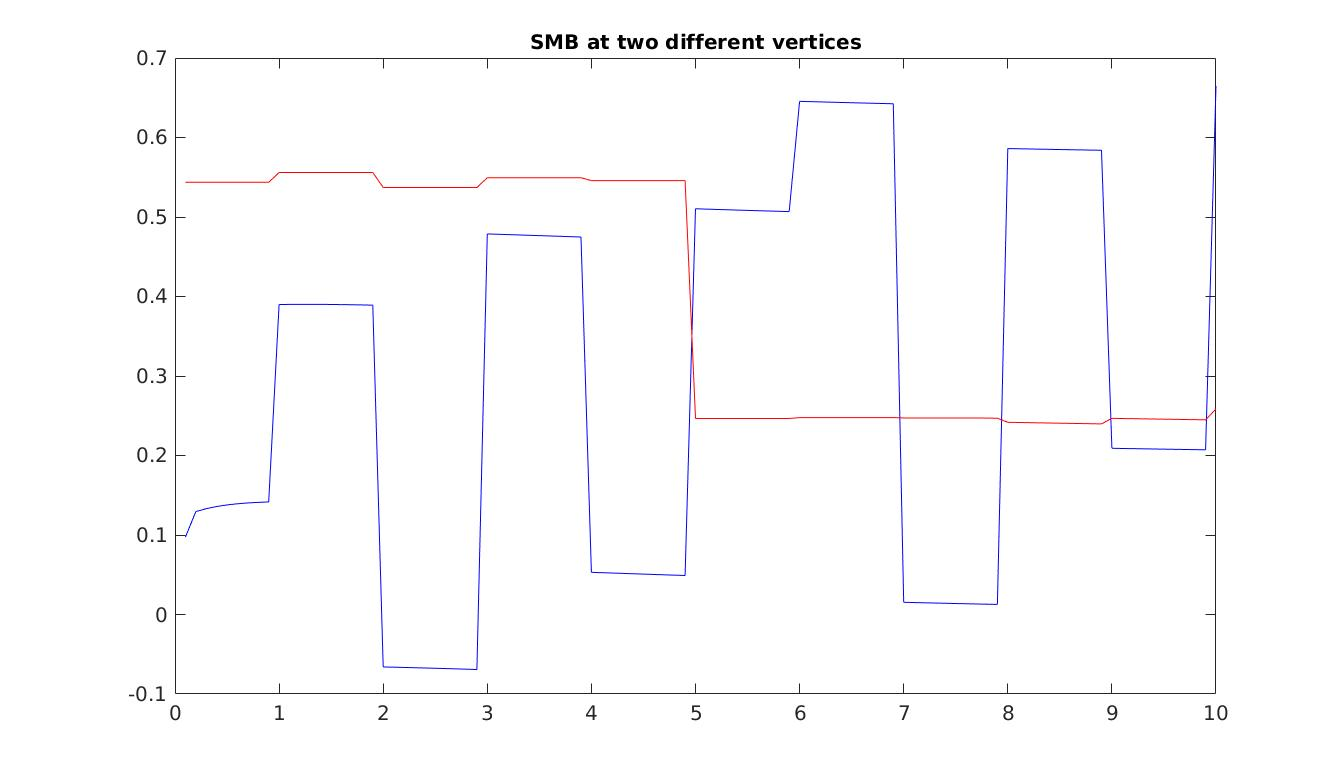
\includegraphics[scale=0.35]{\assetsParentPath/assets/img/using-issm/tutorials/pigstissm/fig3SMBseries.jpg}
	\end{center}
\end{figure}
\begin{figure}
	\begin{center}
		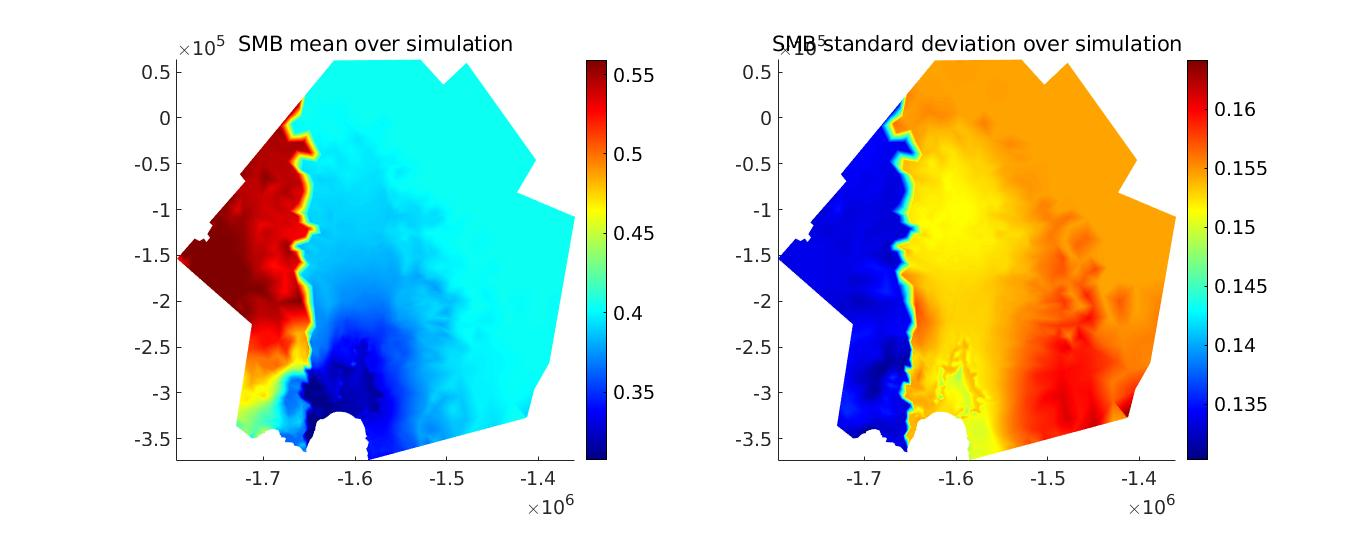
\includegraphics[scale=0.35]{\assetsParentPath/assets/img/using-issm/tutorials/pigstissm/fig4SMBmaps.jpg}
	\end{center}
\end{figure}
%}}}

\subsubsection{Stochastic calving}%{{{
In the last step of this tutorial, we also want to activate stochastic calving. First, we need to specify that calving at the ice front is activated, and specify the background calving values. Notice also that imposing calving means that we need to allow for the ice front to migrate by setting \lstinlinebg|md.transient.ismovingfront| to 1.
Here, we assign the same subdimensions for calving as for SMB. Next, we need to set the covariance matrix for calving. This involves setting the individual standard deviations for the two subdomains, the correlation matrix (here, we set no correlation), and applying Eq. (3). Finally, we modify the \lstinlinebg|md.stochasticforcing| class. We specify that two fields are stochastic \lstinlinebg|[{`SMBarma'}, {`DefaultCalving'}]|. We stack the SMB and calving covariance matrices together, here assuming no correlation between these different fields. As a final note, calving is not an ARMA model, thus its subdimensions must be passed as the default dimensions of the \lstinlinebg|md.stochasticforcing| class.
Set \lstinlinebg|step = 6| in the \lstinlinebg|runme.m| file to execute this step.
%}}}

\subsubsection{Transient run 2}%{{{
We want to launch a second transient run. First, we load the final geometry, masks, and velocities of the previous transient run, and set these as initial conditions for the second transient run. The model is now fully configured for the second transient run. We launch the transient simulation, and plot some results. Again, the plots generated are an example of possible results, which will vary due to the stochastic nature of the model run.
Set \lstinlinebg|step = 7| in the \lstinlinebg|runme.m| file to execute this step.
\begin{figure}[hbt!]
	\begin{center}
		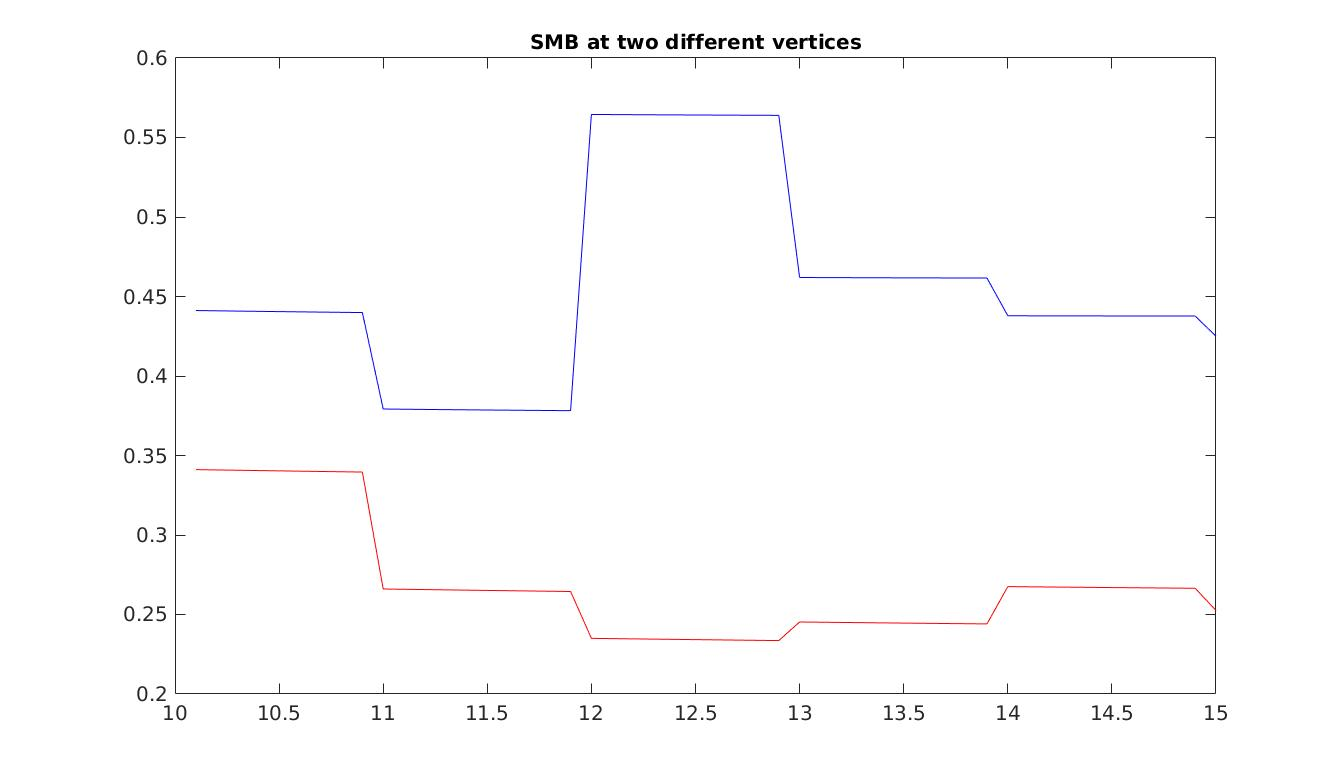
\includegraphics[scale=0.35]{\assetsParentPath/assets/img/using-issm/tutorials/pigstissm/fig5SMBseries.jpg}
	\end{center}
\end{figure}
\begin{figure}[hbt!]
	\begin{center}
		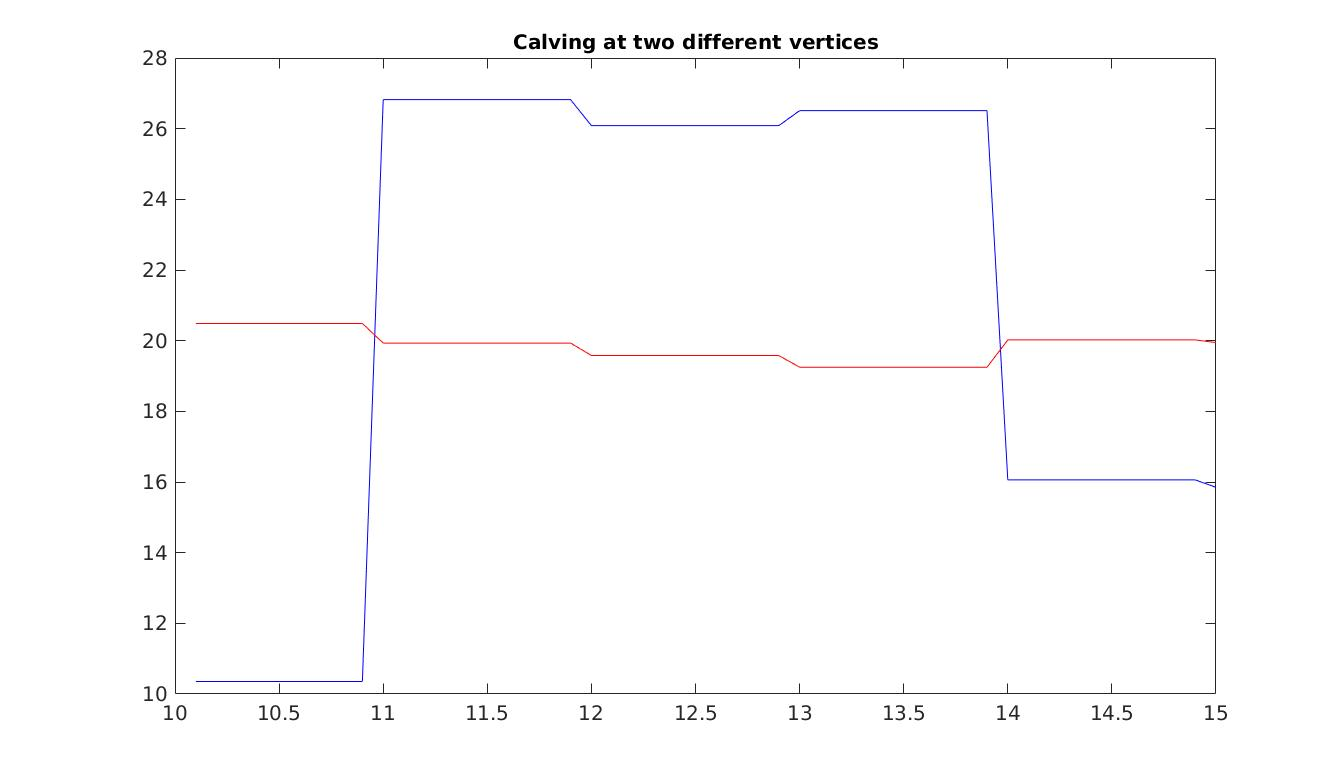
\includegraphics[scale=0.35]{\assetsParentPath/assets/img/using-issm/tutorials/pigstissm/fig6calvingseries.jpg}
	\end{center}
\end{figure}
%}}}

\clearpage % Make sure all figures are placed before next section
